% ---------- SECTION III - FOUNDATIONS ----------
% - [] Authentication and Authorisation
% - [] Password-based auth

\section{Foundations}
\label{sec:foundations}

The following chapter explains some basic concepts of web authentication and digital identities.

% ---- Authn and Authz ----
\subsection{Authentication and Authorisation}
\label{subsec:authn_authz}

\ac{authn} and \ac{authz} are concepts present in virtually every protected \ac{it} ressource.
The former describes the process of identifying a user by verifying their digital identity, hence checking their \emph{authenticity}. Oftentimes only certain users are \emph{authorized} to access a protected ressource (e.g. specific parts of a website, sensitive data etc.). Therefore, an authorization has to take place both to ensure that the correct information is distributed to each user, and that no one without permission is able to manipulate data.\\
The most common and widespread type of web authentication is the so-called password-based authentication. In this case a user has to provide a \emph{username} (oftentimes an e-mail address, as these are globally unique) and a \emph{password} or \emph{passphrase}, a secret string only known to the user.\\
Only the correct combination of username and password grants access to the protected resource.\\
\\
In the above case the password is also referred to as an \emph{authentication factor}, of which there are three categories \cite{turner2016}:

\begin{description}
    \item[Knowledge factors] Something (only) the user knows like a password/-phrase or a \ac{pin}
    \item[Ownership factors] Something the user owns like a smart card or a \ac{totp} token
    \item[Inherence factors] Mostly biometric factors like fingerprints
\end{description}

This classification allows for a basic evaluation of possible \ac{authn} factors: While inherence factors are almost always available (the user carries them around), they often require special hardware like fingerprint sensors and are therefore not best suited for web authentication.\\
Ownership factors on the other hand are less resilient against (physical) theft - if the smartphone or hardware token is stolen, the attacker could authenticate.\\
The security of passwords and other knowledge factors is dependent on the users and how they store and generate them. Reusing passwords or using obvious, common or dictionary-based strings is undeniably less secure than using long, randomly generated ones stored in a password manager \cite{lyastani2018,hunt2011,hunt2018c}. Therefore, application developers have little influence on the security of possibly very important accounts, and if they try to enforce strong passwords by using arbitrary requirements, this can easily backfire \cite{hunt2017} and just decrease usability instead of increasing security. For that reason, the \ac{nist} has dropped all recommendations to use password complexity requirements and instead suggests to rely on length and black lists of known (and therefore insecure) passwords \cite{nist}.

% ---- MFA ----
\subsection{Multi-Factor Authentication}
\label{subsec:mfa}

% - Often \ac{2fa} using \ac{hotp} or \ac{totp}
% - Also possible with key files
% - Only guessing or stealing the password is not enough
To counter the security problems inherent to each single factor, \ac{mfa} can be used for further securing any authentication process by requiring more than one factor. Often this is realized as a \ac{2fa} using a normal password (knowledge factor) as the first, and some kind of \ac{otp} (for example \ac{totp}, \ac{hotp} or an SMS/eMail-Code) as the second.\\
In this case knowing the password of an account is not sufficient for logging in; a possible attacker would also have to get access to the device generating or receiving the second factor, often the users phone (ownership factor) \cite{statista_2fa,hunt2018a}.\\
It is important for \ac{mfa} in general that at least two of these factors are in different categories (e.g. a knowledge and an ownership factor) and at least one of them is not reusable (i.e. a \ac{otp}) \cite{nist,turner2016}.\\
\\
Using multiple factors can protect accounts against standard brute-force attacks like credential stuffing, where an attacker tries many combinations of known usernames and popular passwords.\\
However, \ac{mfa} is not a reliable protection against phishing attacks \cite{lyastani2020}, because a malicious site can easily fake an input field for \acp{otp}.


% ---- Federated Auth ----
% \subsection{Federated Authentication}
% \label{subsec:fed_auth}

% - Federated Identity Providers
% - Shibboleth, Kerberos
% - OAuth, OpenID, Login with Google/Facebook
% - Target resource (SP) never knows the password
% - User only has to remember a single password for many services, without increased risk


% ---- FIDO2 \& WebAuthn ----
\subsection{FIDO2 Overview}
\label{subsec:fido2_webauthn}

\ac{fido2} aims to provide a strong authentication factor (either as single factor for passwordless login or in a \ac{mfa} setting) using hardware keys, so called \emph{authenticators}. Those can be on the device itself (for example using \emph{Windows Hello}, Apples \emph{TouchID} or a \ac{tpm} chip), and therefore be \emph{internal} authenticators. The alternative are external or \emph{roaming} authenticators, often realised as USB keys or \ac{nfc} cards.\\
The party providing the protected ressource (e.g. a website or other web application) is referred to as \emph{relying party}.\\
The \ac{fido2} Framework consists mainly of two components: The \emph{WebAuthn} web \ac{api}, standardized by the \ac{w3c}, is the interface between the browser or \ac{os} and the authentication servers of the relying party \cite{webauthn_standard}. WebAuthn is currently supported by the Windows 10 and Android \acp{os} as well as by the Google Chrome, Mozilla Firefox, Microsoft Edge and Apple Safari web browsers \cite{fido2_webauthn}.\\
The second part is the \ac{ctap2} protocol that is responsible for connecting roaming authenticators to the clients device (e.g. a smartphone, laptop or personal computer) \cite{fido2_overview,fido2_ctap}.\\

\begin{figure*}[ht]
    \centering
    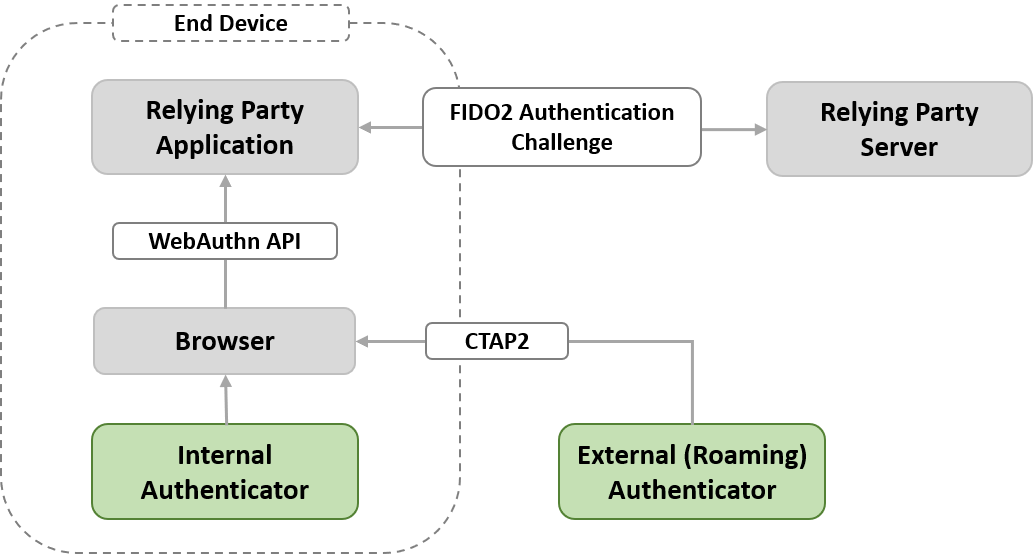
\includegraphics[width=1.8\columnwidth]{Figures/fido2_webauth_ctap_flow.png}
    \caption[FIDO2 Authentication Flow]{FIDO2 WebAuthn \& CTAP2 Authentication Flow}
    \label{fig:fido2_webauth_ctap_flow}
\end{figure*}

As seen in figure \ref{fig:fido2_webauth_ctap_flow}, the \ac{rp} will never know what kind of authenticator was used - as long as it can communicate over WebAuthn (or indirectly over \ac{ctap}).